\documentclass{article}

\usepackage[utf8]{inputenc}
\usepackage[german]{babel}
\usepackage[
    a4paper, top=2.5cm, bottom=2.5cm, left=2.5cm, right=2.5cm, marginparwidth=1.75cm
]{geometry}
\usepackage{amsmath}
\usepackage{amsfonts}
\usepackage{enumitem}
\usepackage[
    colorlinks=true, 
    citecolor=black,
    filecolor=black,
    linkcolor=black,
    urlcolor=blue
]{hyperref}
\usepackage{graphicx}
\usepackage{amssymb}
\usepackage{float}
\usepackage{siunitx} \sisetup{locale = DE}
\usepackage{pdfpages}
\usepackage{multirow}
\usepackage[
    tocskip=0.1\baselineskip, skip=0.7\baselineskip, parfill
]{parskip}
\usepackage{listings}
\usepackage{fancyhdr}
\usepackage{xcolor}

% Kopf- und Fußzeile
\pagestyle{fancy}
\fancyhf{}
%Kopfzeile mittig mit Kaptilname
\fancyhead[C]{\nouppercase{\leftmark}}
%Fußzeile links bzw. innen
\fancyfoot[L]{\versuchsname}
%Fußzeile mittig (Seitennummer)
\fancyfoot[R]{\thepage}
\renewcommand{\footrulewidth}{0.35pt}

% Hilfs-Commands für Gleichungen
\newcommand{\widespace}{\enspace}
\newcommand{\wideeq}{\widespace = \widespace}
\newcommand{\wideneq}{\widespace \neq \widespace}
\newcommand{\wideapprox}{\widespace \approx \widespace}
\newcommand{\wideleq}{\widespace \leq \widespace}
\newcommand{\widegeq}{\widespace \geq \widespace}
\newcommand{\widele}{\widespace \le \widespace}
\newcommand{\widege}{\widespace \ge \widespace}
\newcommand{\wideiff}{\widespace \iff \widespace}
\newcommand{\wideimplies}{\widespace \implies \widespace}
\newcommand{\pd}[2]{
    \frac{\partial #1}{\partial #2}
}
\newcommand{\result}[2]{
    #1 \, \text{#2}
}

% Markieren von verwendetem Code
\definecolor{codebg}{RGB}{230, 240, 255}
\newcommand{\coderef}[1]{%
    \text{\footnotesize \colorbox{codebg}{\texttt{#1()}}}%
}

% Formatieren von Code im Anhang
\definecolor{codegreen}{rgb}{0,0.6,0}
\definecolor{codegray}{rgb}{0.5,0.5,0.5}
\definecolor{codepurple}{rgb}{0.58,0,0.82}
\definecolor{backcolour}{rgb}{0.95,0.95,0.92}
\lstdefinestyle{mystyle}{
    backgroundcolor=\color{backcolour},   
    commentstyle=\color{codegreen},
    keywordstyle=\color{magenta},
    numberstyle=\tiny\color{codegray},
    stringstyle=\color{codepurple},
    basicstyle=\ttfamily\footnotesize,
    breakatwhitespace=false,         
    breaklines=true,                 
    captionpos=b,                    
    keepspaces=true,                 
    numbers=left,                    
    numbersep=5pt,                  
    showspaces=false,                
    showstringspaces=false,
    showtabs=false,                  
    tabsize=4
}
\lstset{style=mystyle}

% Formatierung von Absätzen
\renewcommand{\baselinestretch}{1.2}

\allowdisplaybreaks

% Allgemeine Infos
\newcommand{\versuchsname}{
    ROE - Röntgenstrahlung: Bragg-Reflexion und Röntgenfloureszenzanalyse
}

\newcommand{\githuburl}{
    \url{https://github.com/WeinSim/P3B}
}

% Titel und Autor
\title{\versuchsname}
\author{Simon Weinzierl, Yannic Werner}

\begin{document}

\maketitle

\begin{center}
    Physikalisches Fortgeschrittenenpraktikum P3B
    nach der Studienordnung für Studienbeginn bis WS 2022/23
\end{center}

\vspace*{6cm}

\begin{center}
    \footnotesize
    Alle Teile dieses Dokuments (Vorbereitung, Protokoll, Auswertung) wurden
    von beiden Teilnehmern in gleichen Teilen und ohne fremde Hilfe bearbeitet.
    Sofern fremde Quellen verwendet wurden, sind diese angegeben.

    Der \LaTeX-Code ist auf GitHub unter \githuburl verfügbar.
    
    © Alle Rechte vorbehalten.
\end{center}

 % LMU-Siegel
\AddToShipoutPicture*{
    \put(315,0){
        \parbox[b][5cm]{5cm}{
            
\includegraphics[width=10cm]{Abbildungen/Siegel_LMU.pdf}
        }
    }
}

\newpage

% Inhaltsverzeichnis
\tableofcontents

\newpage

% Literatur
\bibliographystyle{alpha}
\bibliography{literatur}

\newpage


\section{Vobereitung}

\subsection{Physikalischer Hintergrund}

\subsubsection{Röntgenröhre}

\cite{medp}

Röntgenstrahlung entsteht durch die Geschwindigkeitsänderung geladener Teilchen. Dabei wird die Rönt-genstrahlung durch das Abbremsen energiereicher Elektronen in einer Röntgenröhre erzeugt.

Folgend ist der Aufbau einer Röntgenröhre skizzenhaft dargestellt:

\begin{figure}[H]
    \centering
    \includegraphics[width=0.7\linewidth]{Abbildungen/Röntgenröhre.pdf}
    \caption{Skizzenhafte Röntgenröhre}
\end{figure}

Durch das Anlegen einer Heizspannung von einigen Volt an der Kathode treten, bedingt durch den thermoelektrischen Effekt, schwach oder gar nicht gebundene Elektronen aus der Heizwendel aus. Durch die angelegte Anodenspannung werden die Elktronen von der Kathode zur Anode beschleunigt und treffen anschließend auf die Anode.

Durch die Bremsstrahlung und durch die Wechselwirkungen unter den einzelnen Elektronen kommt es zur Entstehung von Röntgenstrahlung. Deren Überlagerung bildt das emittierte Röntgenspektrum. Die Eigenschaften und die Entstehung von Bremsstrahlung und der charakteristischen Strahlung werden im Kapitel 1.1.3 genauer beleuchtet. 

\subsubsection{Linienspektrum eines Stoffe, Schalenmodell, mögliche Übergänge (Quantenmechanik)}

\cite{chemie.de}
\cite[1050--1051]{Physik}
\cite{studyfix}

Ein Linienspektrum ist ein Strahlungsspektrum, welches voneinander getrennte, diskrete Linien zeigt. Das können zum Beispiel Absoroptions- oder Emissionlinien in Lichtspektren sein. Jedoch weisen auch manche Teilchenstrahlungen, wie die Alphastrahlung, Lininespektren auf. Daraus kann man ableiten, dass auch Teilchen diskrete kinetische Energien haben.

Jedes Material (Atom, Molekül) hat dabei chrakteristische, diskrete Energieniveaus, auf welchen sich die Elektronen befinden können. Der Wechsel von einem Energienievau auf ein anderes erfolgt dabei durch Aufnahme / Abgabe eines Pohotons. Aus der Energiedifferenz lässt sich dann die zugehörige Wellenlänge über folgende Formel bestimmen: $\lambda=\frac{c}{v}$.

Ein angeregtes Atom oder Molekül befindet sich immer nur sehr kurz in seinem angeregten Zustand. Es fällt nach einer sehr kurzen Zeitspanne wieder in einen tieferen Energiezustand zurück. Die ausgesandten Photonen erscheinen dann mit einer ganz bestimmten Energie als Emissionslienien auf einem Spektrum. So entstehen chrakteristische Spektren, wie zum Beispiel das Spektrum von Wasserstoff oder Helium.


Das Schalenmodell ist ein Modell, um den Aufbau von Atomen zu beschreiben. Das Schalenmodell basiert hierbei auf dem Bohr'schen Atommodell. Im Atomkern befinden sich die Protonen und Neutronen. Die negativ geladenen Elektronen bewegen sich in Schalen um den positiv gelandenen Kern. Folgende Skizze soll das Schalenmodll verdeutlichen:

\begin{figure}[H]
    \centering
    \includegraphics[width=0.3\linewidth]{Abbildungen/Schalenmodell.pdf}
    \caption{Schalenmodell}
\end{figure}

Die Schalen haben, wie in der Abbildung ersichtlich, unterschiedlich Abstände zum Kern. Die Schalen werden von innen nach außen mit unterschiedlichen Buchstaben bezeichnet, beginnend mit der K-Schale, L-Schale und M-Schale. Dabei haben die Schalen unterschiedlich viel Platz für Elektronen  Über die Formel $e=2n^2$ lässt sich die maximale Anzahl an Elektronen für jede Schale bestimmen.

Jedoch hat das Schalenmodell auch Grenzen. Will man Elemente mir mehr als 20 Elektronen beschreiben, so ist das Schalenmodell zur Beschreibung nicht mehr geeignet!


Der Zusammenhang mit der Quantenmechanik ist nun leicht hergestellt. Die Quantenmechanik besagt, dass ein Elektron in einem Atom nur auf bestimmen Energieniveaus existieren kann und nicht zwischen den Niveaus! Wie oben bereits beschrieben können also folgende Aussagen getroffen werden:
    \begin{enumerate}[label=\arabic*.]
        \item Abstieg: ein Photon wird emittiert (von $E_2$ nach $E_1$)
        \item Aufstieg: ein Photon wird absorbiert
    \end{enumerate}
Die Energie des Photons wird also genau durch den Energieunterschied der beiden Zustände beschrieben: 
\[
    E_\text{Photon} \wideeq E_\text{oben} - E_\text{unten}
    \wideeq h f \wideeq \frac{h c}{\lambda} 
\]

mit $h$ als Planksches Wirkungsquantum, $f$ als Frequenz, $\lambda$ als Wellenlänge und $c$ als Lichtgeschwindigkeit.

Folgende Aussagen lassen sich also zusammenfassend treffen:
\begin{enumerate}[label=\arabic*.]
        \item Die Energiedifferenzen werden durch Linienspektren beschrieben
        \item Die Energiedifferenzen entstehen durch Übergänge von Elektronen zwischen den unterschiedglichen Energieniveaus
        \item Jedem Übergang ist eine chrakteristische Linie zugeordnet
        \item Jedes Atom wird durch ein charakteristisches Linienspektrum beschrieben
    \end{enumerate}

Beispiel Wasserstoffatom:
\begin{itemize}
    \item Lyman-Serie: Übergang nach $n=1$
    \item Balmer-Serie: Übergang nach $n=2$
    \item Paschen-Serie: Übergang nach $n=3$
    \item Bracket-Serie: Übergang nach $n=4$
    \item Pfund-Serie: Übergang nach $n=5$
\end{itemize}
Hier ist wohl die Balmer-Serie die bekannteste Serie, da hier das Linienspektrum mit dem bloßen Auge sichtbar ist.

\subsubsection{Röntgenstrahlung (Bremsstrahlung, chrakteristische Strahlung)}

\cite[1010--1011; 1384]{Physik}
\cite{leifiphysik_B}
\cite{leifiphysik_C}

Wie bereits in Kapitel 1.1.1 erwähnt, wird in diesem Kapitel die Bremsstrahlung und die charakteristische Strahlung genauer betrachtet.

Die Kathode in der Röntgenröhre beschleunigt die Elektronen auf eine Geschewindigkeit von circa $0,35c$. Die ausgetretenen Elektronen treffen nun mit dieser hohen Geschwindigkeit auf die Anode in der Röntgenröhre. Durch das extreme Abbremsen der Elektronen entsteht elektrische Strahlung, die sogenannte Bremsstrahlung. Je stärker die Elektronen abgebremst werden, umso mehr Strahlung senden diese aus. Da nicht alle Elektronen gleich stark abgebremst werden, besitzen die Photonen der Bremsstrahlung unterschiedliche Wellenlängen. Dadurch ist das Spektrum der Bremsstrahlung ein kontinuierliches Spektrum. Die minimale Wellenlänge wird häufig als $\lambda_{gr}$ bezeichnet. Die minimale Wellenlänge lässt sich durch folgende Formel bestimmen:
\[
    \lambda_{gr}=\frac{hc}{eU}
\]

wobei $h$ das Planksche Wirkungsquantum, $c$ die Lichtgeschwindigkeit, $e$ die Elementarladung und $U$ die Beschleunigungsspannung ist.

Aus der Formel lässt sich ableiten, dass die minimale Wellenlänge und die Beschleunigungsspannung indirekt proportional zueinander sind. Mit steigender Beschleunigungsspannung sinkt die minimale Wellenlänge.

Abschließend lässt sich also zur Bremsstrahlung folgendes zusammenfassen: das kontinuierliche Spektrum entsteht durch das Abbremsen der ausgesandeten, beschleunigten Elektronen der Kathode. Durch das unterschiedlich starke Abbremsen der Elektronen werden Photonen mit unterschiedlichen Energiewerten entsandt, wobei die minimale Wellenlänge / die maximale Photonenenergie von der Beschleunigungsspannung der Röntgenröhre abhängen.

Neben der Bremsstrahlung tritt bei ausreichend großer Beschleunigungsspannung auch ein charakteristisches Linienspektrum auf. Diese Röntgenstralhung ist jedoch nur bei höheren Ordnungszahlen beobachtbar. Das liegt daran, dass Atome mit höherer Ordnungszahl zahlreiche Atome in den äußeren Elektronenschalen haben. Diese sind nicht so stark an den Atomkern gebunden und können somit leichter austreten als Elektronen, welche sich nahe dem Kern befinden. Im folgenden soll die Entstehung der chrakteristischen Stralung stichpunktartig beschrieben werden:
\begin{itemize}
    \item Ein Anode-Atom wird durch ein sehr schnelles Elektron angeregt. Ein Elektron wird folgich auf ein noch freies, höheres Energieniveau angehoben. Auf einer der unteren Schalen entsteht somit eine Lücke. Wie bekannt gehen angeregt Atome nach kurzer Zeit in energetisch günstigere Zustände über. Folglich kann folgendes passieren:
    \item Möglichkeit 1: Ein Elektron der höchsten Schale fällt nun wieder zurück auf die Lücke der untersten Schale. Dabei wird ein Photon emittiert.
    \item Möglichkeit 2: Die Lücke der untersten Schale wird durch ein Elektron auf einer höheren Schale aufgefüllt. Hierbei wird ein Photon emittiert. Die so enstandene Lücke in der höheren Schale wird erneut durch ein Elektron einer Schale darüber aufgefüllt. Es wird wieder ein Photon emittiert. Dieser Vorgang läuft so lange ab, bis wieder alle Schalen aufgefüllt sind, bis auf die äußerste Schale.
\end{itemize}

Zusammenfassend lässt sich also sagen, dass das Röntgen-Spektrum durch charakteristische Strahlung identifiziert werden kann. Elektronenübergänge zwischen den unterschiedlichen Schalen der Atome sind die Ursache für das Auftreten der charakteristischen Strahlung.

\subsubsection{Zustandekommen der charakteristischen Strahlung im Röntgenspektrum ($K_\alpha$, $K_\beta$)}

\cite{leifiphysik_C}

Wie bereits in den vorangegangenen Kapiteln beschrieben treten neben dem Spektrum der Bremsstrahlung auch charakteristische Linien im Spektrum auf. Diese Linienspektren sind die Folgen von Übergängen zwischen den Energieniveaus. 

Wie in 1.1.3 beschrieben ensteht durch das Anregen eines Atoms durch ein Elektron eine Lücke auf einer der unteren Schalen. Diese freie Lücke muss nun wieder neu besetzt werden. Hierfür gibt es zwei chrakteristische Mögklichkeiten.

\begin{enumerate}
    \item Die Lücke auf der K-Schale wird durch ein Elektron der M-Schale aufgefüllt. Folglich wird ein Photon emittiert. Dies würde der $K_{\beta}$-Strahlung entsprechen
    \item Wird die Lücke auf der K-Schale durch eine Elektron der L-Schale aufgefüllt und dabei ein Photon emittiert, so spricht man von einer $K_{\alpha}$-Strahlung
\end{enumerate}

\begin{figure}[H]
    \centering
    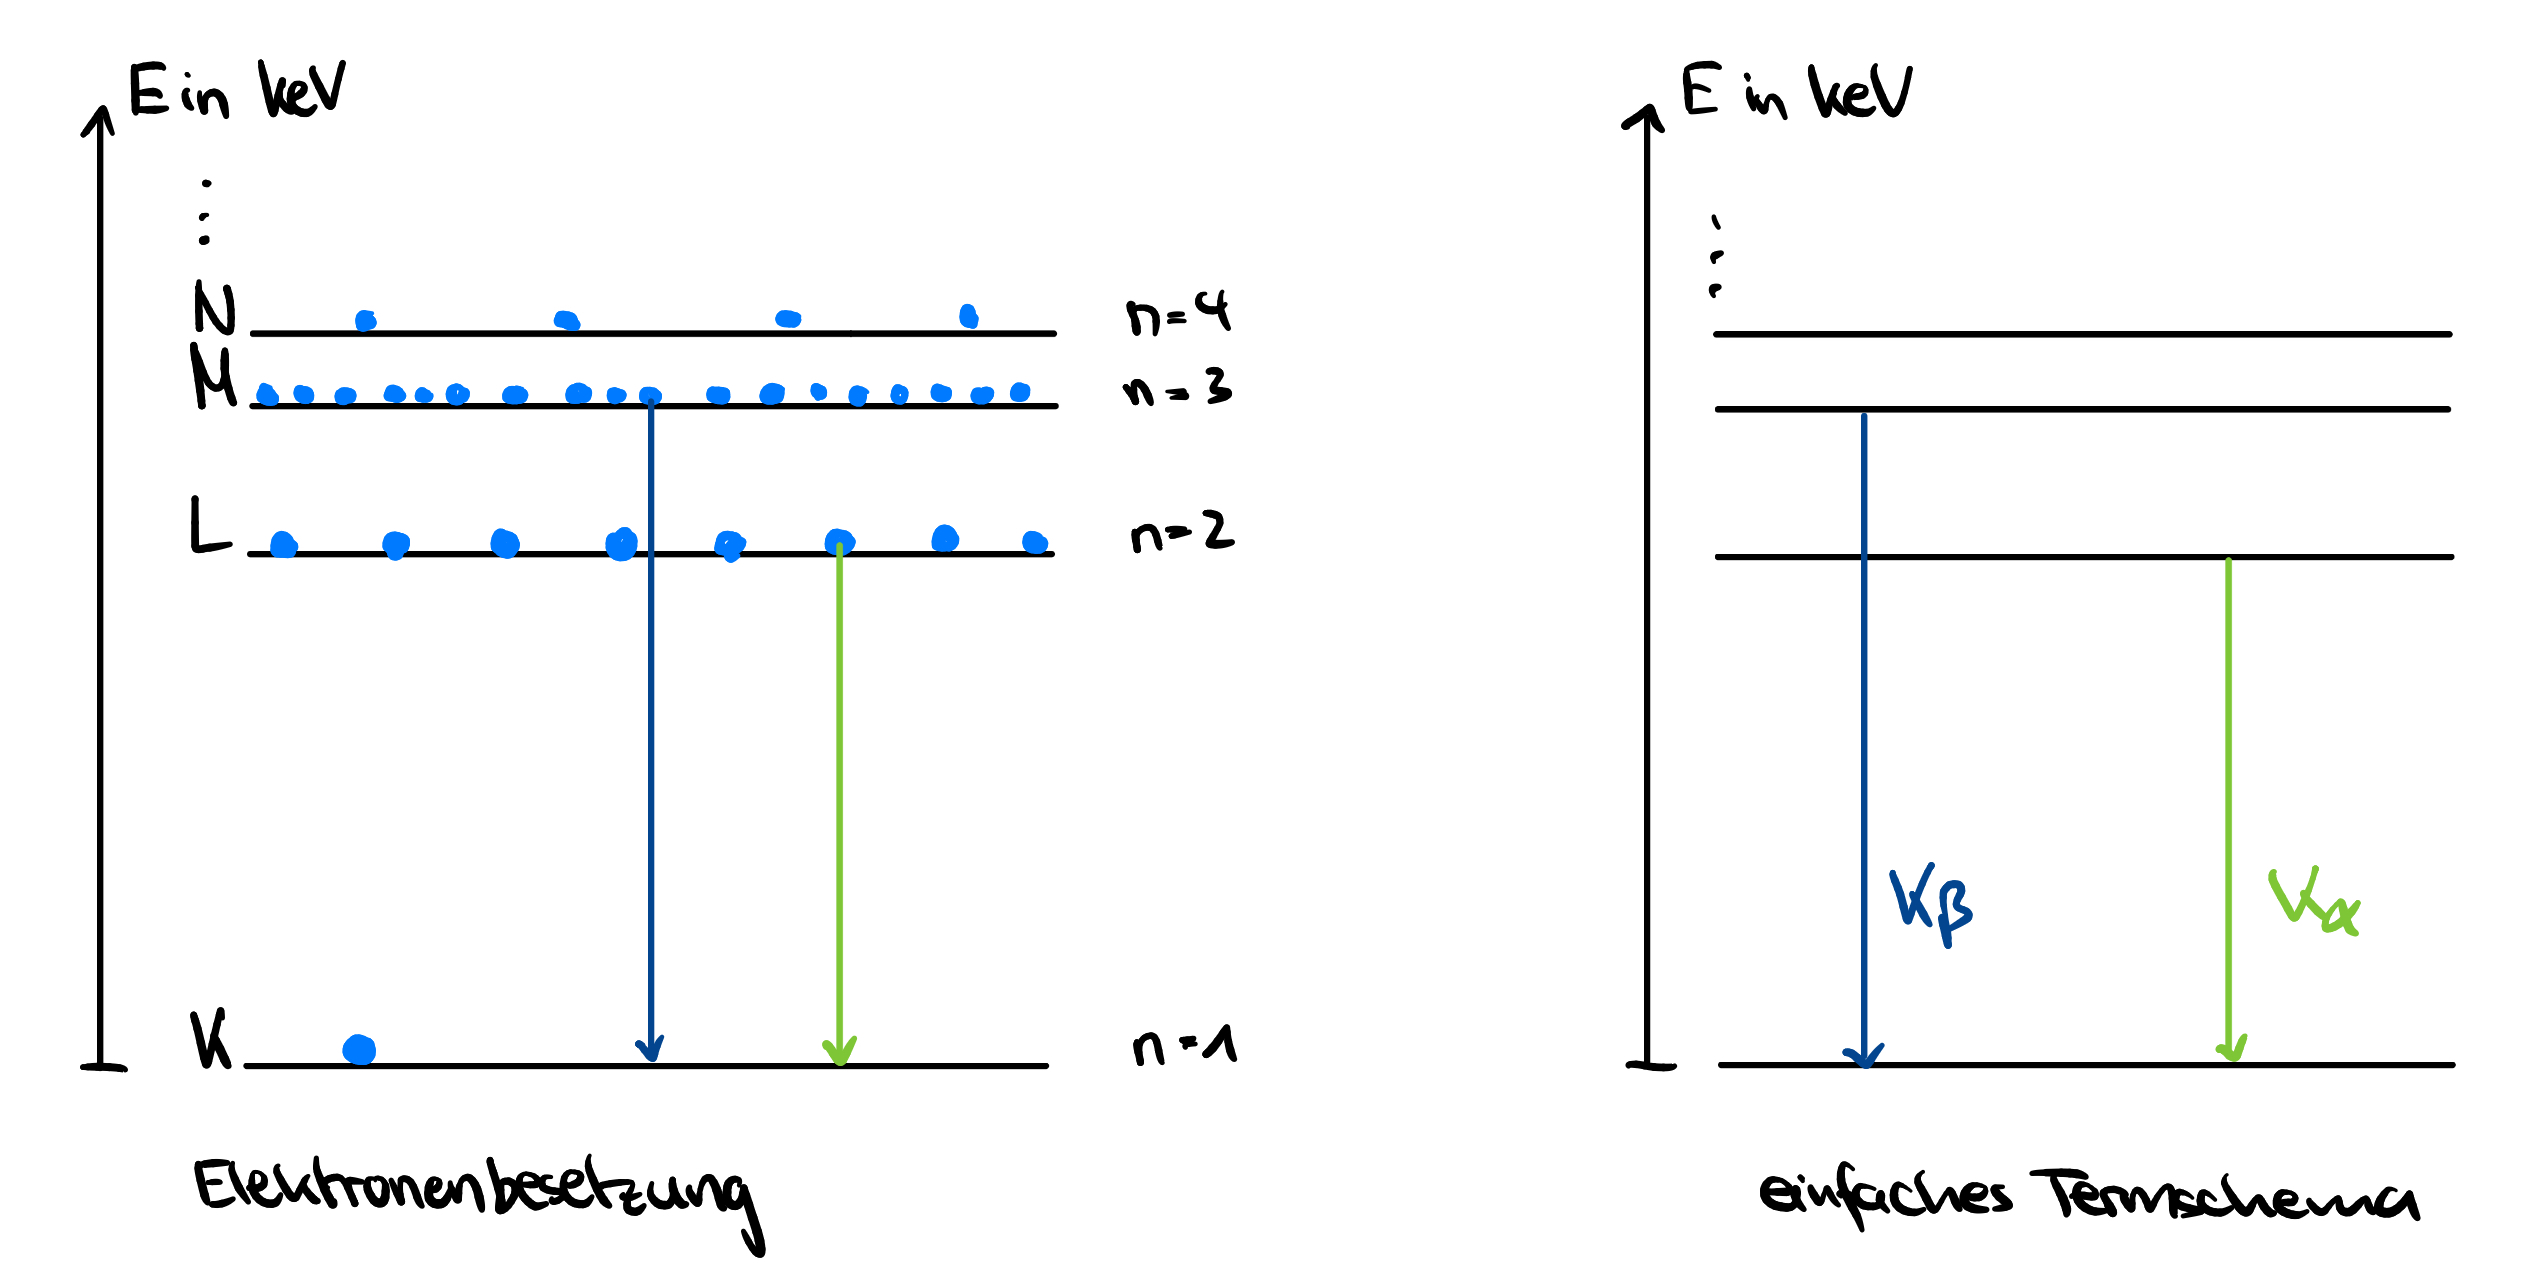
\includegraphics[width=0.6\linewidth]{Abbildungen/Entstehung_R.Strahlung.jpeg}
    \caption{Entstehung der charakteristischen Röntgenstrahlung}
\end{figure}

Der Einfachheit wurden beide Strahlungen in eine Skizze gezeichnet. Das bedeutet jedoch nicht, dass beide Strahlung gleichzeitig auftreten können!

Wie also ersichtlich, ist die Bezeichung der Strahlung davon abhängig, welche Schale wieder besetzt wird. 
Die so neu entstandenen Lücken auf den darüberliegenden Schalen werden erneut durch Elektronen darüberliegender Schalen besetzt. 


\subsubsection{Bragg Reflexion (Netzebenen einer Kristallstruktur, Streuung, Interferenz, Bragg-Winkel, Gleichung)}

\cite{Physik} [1302]

Netzebenen werden verwendet, um die Streuung von Strahlung an Kristallgittern zu verwenden. Eine solche Netzebene wird definiert, beziehungsweise aufgesapnnt durch zwei linear unabhängige Gittervektoren. Im Beispiel eines Kristalls: ein solcher ist von solchen Netzebenen volsltändig durchzogen. Diese Netzebenen laufen auf den drei Achsen durch einen Gitterpunkt. Zudem lassen sich weitere Netzebenen zeichen. Das sind jedoch genau so viele, dass auf jeder der drei Achsen alle Gitterpunkte der Achse auf einer Netzebene liegen. 

Der Abstand zwischen zwei Netzebene lässt sich mit folgender Gleichung darstellen,
\[
    d_{hkl} \wideeq 2 \pi \frac{1}{G_{hkl}}
\]

wobei $G_{hkl}$ der Betrag des Gittervektors $\mathbf G_{hkl}$ ist.
Der Vektor $\mathbf G_{hkl}$ hat die Komponenten $h$, $k$, und $l$ und steht senkrecht auf den so bezeichneten Netzebenen.
Das Triplet der teilfremden Zahlen / der Indizes wird als Miller'sche Indizes bezeichnet, welche einen Punkt in den Netzebenen klar definieren.

Trifft eine Welle mit Wellenvektor $\mathbf k_0$ auf einen Kristall und wird an
diesem gestreut, so lässt sich die gestreute Welle mit dem Wellenvektor $\mathbf k$
beschreiben. Der Streuvektor wird folglich beschrieben durch
$\mathbf K = \mathbf k - \mathbf k_0$. Im Folgenden wird $\mathbf K$ nun mit
$\mathbf G$ ersetzt.
Nimmt man nun den Betrag der Gleichung, so kann man die Bragg-Gleichung aufstellen,
\[
    K \wideeq G_{hkl} \wideeq \frac{2\pi}{d_{hkl}} \wideeq 2 k_0 \sin \theta
\]

woraus die Gleichung
\[
    \lambda \wideeq 2 d_{hkl} \sin \theta \wideeq 2 d \sin \theta
\]
folgt, wobei $\theta$ der eingechlossene Winkel zwischen einfallendem und abgestrahltem Strahl ist.

An dieser Gleichung lässt sich erkennen, dass sich die Wellen so verhalten, als würden sie an den Netzebenen reflektiert werden. Aus der Streubedingung lässt sich nun folgern, dass für konstruktive Interferenz zwischen den an der Ebeneschar reflektierten Wellen gerade eine Wellenlänge $\lambda$ oder eine vielfaches der Wellenlänge liegen muss.

Betrachtet man einen großen Einkristall, so lässt sich feststellen, dass neben der Primärreflexion auch die Bragg-Refelxion auftritt. Beide Reflexionen überlagern sich und bilden zusammen ein Feld stehender Wellen. Mit einem solchen Feld an stehenden Wellen lassen sich experimentell Gitterfehler feststellen

\subsubsection{Duane-Huntsches-Verschiebungsgesettz, Erklärung der Abhängigkeit zwischen Grenzwellenlängen und Röhren-Hochspannung mit einfachen quantenmechanischen Über-legungen)}

\cite{spektrum}

Das Gesetz beschreibt die umgekehrte Proportionalität zwischen minmaler Wellenlänge und der Beschleunigungsspannung beim inversen Photoeffekt. Mathematisch ist das Duane-Huntsche Verschiebungsgesetz wiefolgt beschrieben:

    \[
        \lambda_{min}U=\frac{\hbar c}{e}=const.
    \]

    Aus dieser Gleichung lässt sich ableiten, dass zur Erzeugung einer Bremsstrahlung eine bestimmte Mindestbeschleunigungsspannung notwendig ist.  Möchte man es anders formulieren, so könnte man sagen, dass bei konstantem $\lambda$ ein kontinuierliches Röntgensoektrum ergibt.

\subsubsection{Moseleysches Gesetz (Herkunft, Grundannahmen, ...)}

\cite{chemie.de_2}

Dieses Gesetz beschreibt die Lage der $K_\alpha$-Linie im kontinuierlichen Röntgenspektrum - also die Linie, welche den Übergang eines Elektrons von der L-Schale zur K-Schale entspricht. Entdeckt wurde das Gesetz bei durch die präzise Messung der Röntgenstrahlung für verschiedene Elemente. Es wurde festgestellt, dass die Frequenz nicht von der Atommasse, von der Ordnungszahl abhängt.

Dabei ist der Zusammenhang zwischen der Wellenlänge, der Röntgenstrahlung und der Ordnungszahl gegeben durch:

    \[
        \frac{1}{\lambda}=\overline{v}=R_\infty(Z-K)^2(\frac{1}{n_1^2}-\frac{1}{n_2^2})
    \]

Wie ersichtlich, ist die Fromel eine Erweiterung der Ryberg-Formel. Für den speziellen Übergang eines Elektrons von der L-Schale in die K-Schale, also den $K_\alpha$-Übergang, lässt sich die Formel folgend umschreiben,

    \[
        \overline{v}_K\alpha=R_\infty(Z-1)^2(\frac{1}{1^2}-\frac{1}{2^2})=R_\infty(Z-1)^2\frac{3}{4}
    \]

wobei $Z$ die Ordnungszhal des Elements ist.

\subsubsection{Spektrallinien (Absorptions- und Emissionsspektrum)}

\cite{chemie.de_3}

Spektren und Spektrallinien treten durch Energieübergänge von Elektronen in Atomen auf. Dabei unterschiedet man zwischen Emissions- und Absorptionsspektren.

Dabei beschreibt das Emissionsspektrum einen Elektronenübergang von einem höheren Energieniveau ein ein niedrigeres Energieniveau. Durch das Herunterfallen des Elektrons wird ein Photon emittiert. Die Energie des Photons wird dabei beschrieben durch die Energiedifferenez der beiden Niveaus:

    \[
        E=E_{oben}-E_{unten}
    \]

Das Absorptionsspektrum beschreibt den Übergang eines Elektrons von einem unteren Zustand auf einen höheren. Die geschieht durch die Absorption eines einfallenden Photons. Hierbei sind aber nicht alle Energien erlaubt, sondern nur diese, welchen den Übergangsenergien entsprechen.

\subsubsection{Fluoreszenz/sekundäre Anregung}

\cite{spektrum_2}

Fluoreszenz beschreibt den Übergang eines Atoms von einem angeregten Zustand un den Grundzustand. Dabei werden jedoch meherere dazwischenliegende Zustände durchlaufen.

Sekundräre Anregung beschreibt den Prozess, bei welchem ein Atom durch ein anderes Atom angeregt wird. Dies geschieht durch die abgestrahlte Energie eines Atoms, welches von einem angeregten Zustand in den Grundzustand zurückfällt.

Für diese beiden Prozesse ist die Röntgenfluoreszenz ein passendes Beispiel. Hierbei wird ein Atom durch hochenergetische Röntgenstrahlung angeregt. Dabei wird druch den Effekt der sekundären Anregung Röntgenstrahlung emittiert. Das Atom emittiert also Strahlung, wenn es in seinen Grundzustand zurückfällt. Dies geschieht nicht wie bei der Röntgenröhre durch Beschuss, sondern durch die Absorption von Photonen.

\subsubsection{Detektion von Röntgenstrahlung: Geiger-Müller-Zählrohr und Halbleiterdetektor}

Folgend werden zwei Methoden zur Detektion von Röntgenstrahlung betrachtet. Zum einen das Geiger-Müller-Zählrohr und der Halbleiterdetekor.

\begin{enumerate}
    \item Geiger-Müller-Zählrohr: hiermit kann man ionisierte Strahlung nachweisen, vor allem $\alpha$- und $\beta$-Strahlung. Der positiv geladene Zähldraht ist von einem negativen Zählrohrmantel umgeben. Innerhalb des Zylinders herrscht ein elektrisches Feld, welches um den Draht am stärksten ist. Die Elektron-Ion-Paare bewegen sich im elektrischen Feld auf den Draht hin zu. Dabei werde diese stark beschleunigt. Durch die Wechselwirkung von Elektronen und Atomen des Füllgases, bilden sich im Auslösebereich neue Ladungspaare. Folglich wird das ganze Zählrohr von einer Entladung erfasst, also einem Strom, welcher am Widerstand einen Spannungsimpuls auslöst. 
    \item Halbleiterdetektor: aufgrund der Empfindlichkeit sind diese Detektoren optimal geeignet als Strahlungsdetektoren. Trifft ionisierte Strahlung auf einen Halbleiter, überträgt diese Energie an die Elektronen. Diese Elektronen können nun die Bandlücke des Valenzbands überwinden und in das Leitungsband gelangen. Dadruch entstehen Elektronen-Loch-Paare, welche als primäre Ladungsträger für die Detektion genutzt werden. Durch das Anlegen einer Spannung werden dann die erzeugten Elektronen und Löcher dann in entgegengesetzte Richtungen beschleunigt, was einen elektrischen Strom erzeugt. Dieser ist proportionale zur Anzahl der erzeugten Paare und somit zur Energie der einfallenden Strahlung. Dieser Impuls wird anschließend verstärkt, um schlussendlich die Intensität zu bestimmen. Vor allem Siliziumdetektoren finden hierbei Anwendung in der Röntgenspektroskopie. Ihre hohe Präzision und Emfpindlichkeit sind der Grund, weshalb sie häufig Vernwendung in der Wissenschaft finden.
\end{enumerate}

\newpage

%\subsection{Aufgaben aus dem Text}

%    \subsubsection{Teile der jeweiligen Aufgaben}
%[...]


%\newpage

\section{Veruschsablaufplan}

\begin{center}

\end{center}

\subsection{Benötigte Materialien}
    \begin{enumerate}[label=\arabic*.]
        \item Röntgengerät mit Röntgenröhre MO oder CU und Goniometer
        \item Software X-Ray
        \item NaCl-Kristall
        \item Röntgenenergiedetektot
        \item Sensor-Cassy
        \item VKA-Box
        \item Cassy Lab 2
        \item BNC Kabel 1m
        \item HF-Kabel 1m
        \item Tragesatz K-Linie-Fluoreszenz
    \end{enumerate}

\newpage

\subsection{Aufbau der Braggschen Anordnung}   
    \begin{enumerate}[label=\arabic*.]
        \item Kollimator in die dafür vorgesehene Aufnahme einbauen
        \item Goniometer einbauen (darauf achten, dass der Abstand circa 5cm beträgt!)
        \item Flachbandkabel anstecken
        \item Geiger-Müller-Zählrohr in die Sensoraufnahme einsetzen und Zählrohrkabel an die dafür vorgesehene Buchse anstecken
        \item Durch Verschieben des Sensors den Abstand zwischen Tragetasche und Spaltblende auf circa 6cm einstellen
        \item Tragehalter einbauen
        \item Rändelschraibe lösen und Kristall auf den Tisch legen
        \item USB-Anschluss mit PC verbinden
    \end{enumerate}

\newpage

\subsection{Aufbau und Einstellung des Röntgengerätes zur Röntgenfluoreszenzanalyse}   
    \begin{enumerate}[label=\arabic*.]
        \item Mit den unterschiedlichen Knöpfen vertraut machen
        \item Röntgenenergiedetekor am Sensorarm des Goniometers montieren
        \item Abstand zwischen Drehachse und Eintrittsöffnung des Energiedetektors auf circa 5cm stellen
        \item Anschlusskabel für Spannungsversorgung durch Leerkanal des Geräts führen und an die Mini-DIN-Buchse anschließen
        \item Signalausgang des Energiedetektors mit BNC-Kabel an die SIGNAL IN Buchse anschließen
        \item Anschlusskabel nachführen, sodass dieses bei einem Schwenk des Sensors nicht spannt
        \item CASSY mit PC verbinden
        \item SIGNAL PUT mit BNC Kabel mit der VKA-Box auf dem CASSY Sensor verbinden
    \end{enumerate}

\newpage

\subsection{Teilversuch 1: Bragg-Reflexion von Röntgenstrahlung des Molybdän an einem NaCl-Eiskristall}
\begin{enumerate}[label = (\Roman*)]
    \item Ziel: Untersuchung der Winkelabhängigkeit der charakteristischen Röntgenstrahlung des Molybdän
    
    \item Versuchsmethode: Analyse anhand der Bragg-Reflexion an einem NaCl-Einkristall
    
    \item Versuchsskizze:
    
        \begin{figure}[H]
        \centering
        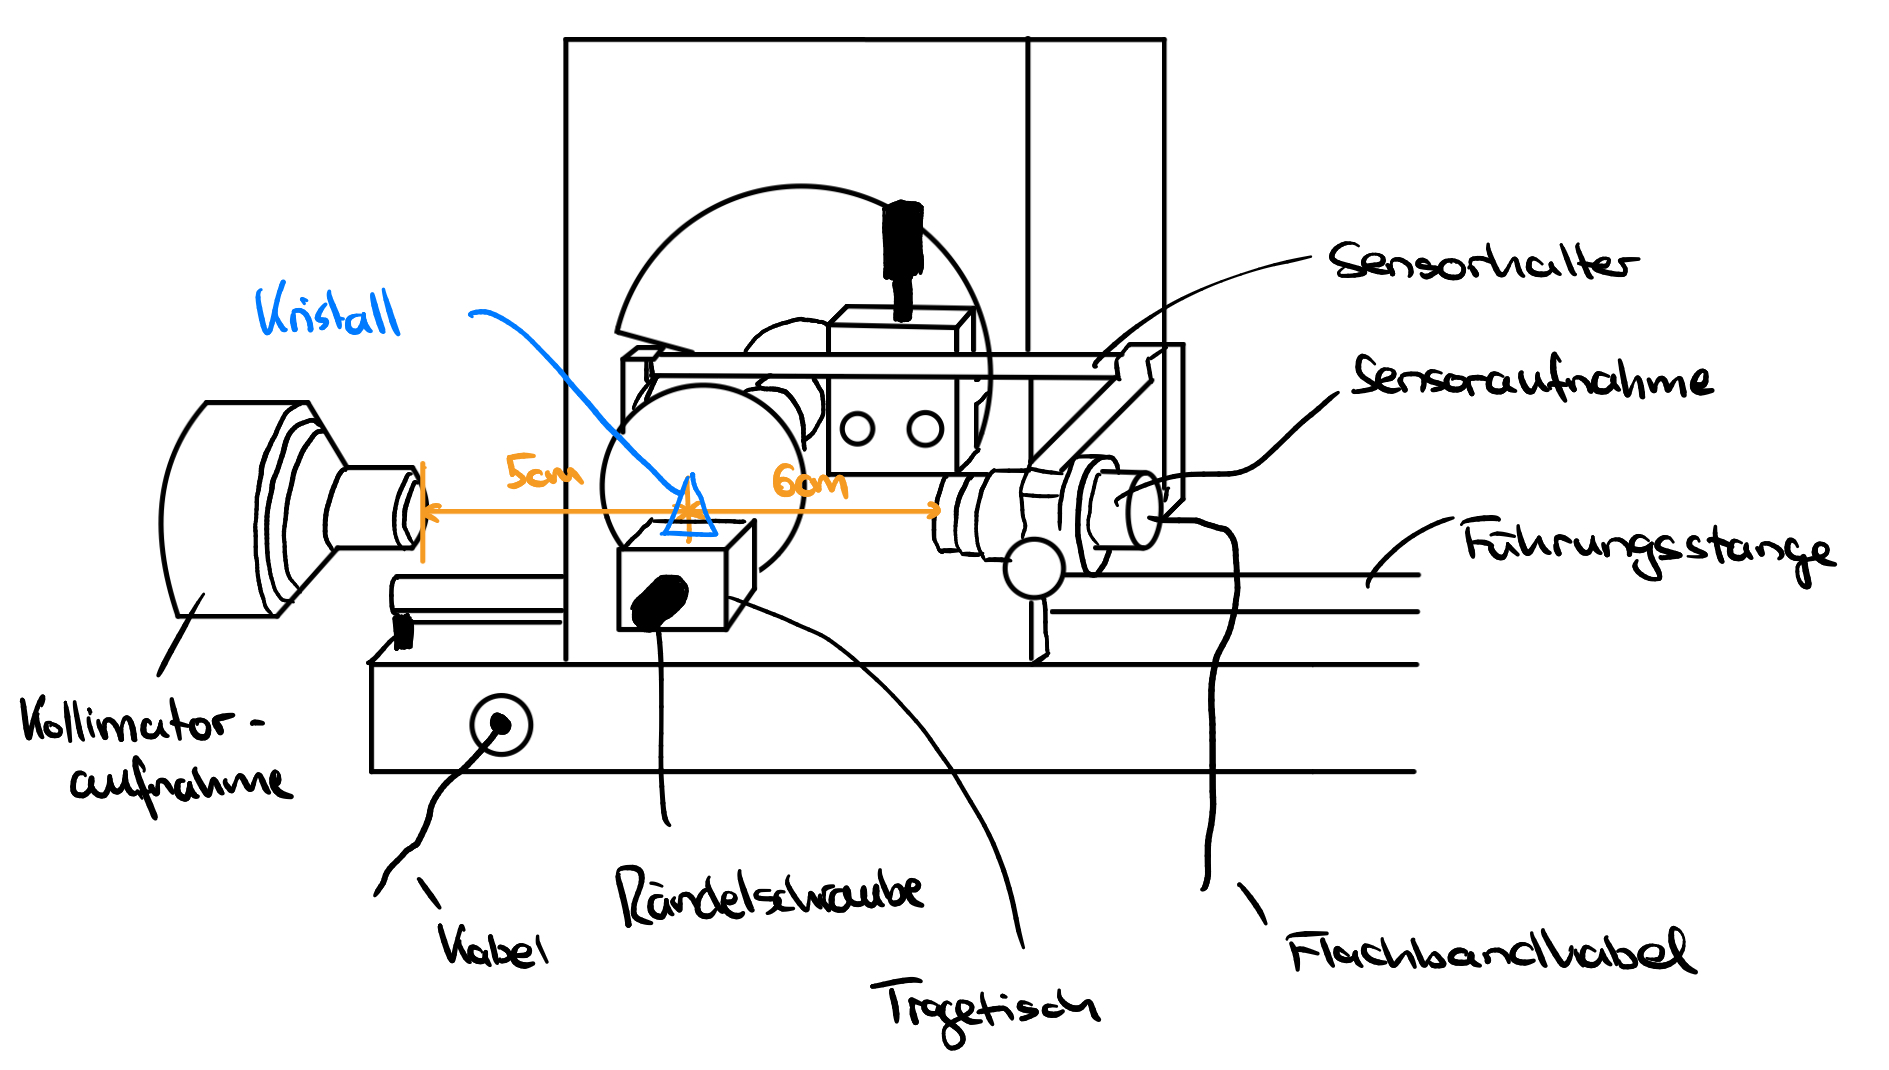
\includegraphics[width=0.7\linewidth]{Abbildungen/Aufbau Bragg Versuche.jpeg}
        \caption{Versuchsskizze Teilversuch 1}
        \end{figure}

    \item Planung der Durchführung
        \begin{itemize}
            \item Computerprogramm Röntgengerät starten und gegebenefalls alte Messdaten löschen
            \item Folgende Einstellungen wählen: $U=35.0kv$, $I=1.00mA$, $\Delta t=10s$ und $\Delta\beta=0.1°$
            \item Targetwinkel einstellen auf: $\beta_{min}=2.5°$ und $\beta_{max}=25.0°$ $\to$ $2\vartheta$-Kopplung von Target und Sensor
            \item Kristall einmessen, um $2\vartheta$-Kopplung zu gewährleisten
            \item Daten an PC übertragen
            \item Von Zeit zu Zeit den Verlauf prüfen
            \item Messreihe abspeichern
        \end{itemize}

    \item Vorüberlegungen zur Durchführung \& Auswertung
        \begin{itemize}
            \item Den Peakschwerpunkt über das Computerprogramm berechnen lassen
            \item Die Peaks jeweils über die gesamte Breite markieren und den ermittelten Schwerpunkt eintragen. Schwepunkt als Bragg-Winkel in Messtabelle notieren
            \item Messungen und Auswertungen speichern
            \item Berchnen der Wellenlänge nach dem Reflexionsgesetz (Netzabstand $d=282.01pm$)
            \item Mittelwerte über ermittelten Werte bilden und mit Literaturwert vergleichen   
        \end{itemize}
    
\end{enumerate}

\newpage

\subsection{Teilversuch 2: Energiespektrum einer Röntgenröhre in Abhängigkeit der Spannung}
\begin{enumerate}[label = (\Roman*)]
    \item Ziel: Bestimmen des Energiespektrums einer Röntgenröhre
    
    \item Versuchsmethode: Aufzeichnung verschiedener Energiespektren einer Röntgenröhre in Abhängigkeit der Beschleunigungsspannung des Elektronenstrahls.
    
    \item Versuchsskizze:
    
        \begin{figure}[H]
        \centering
        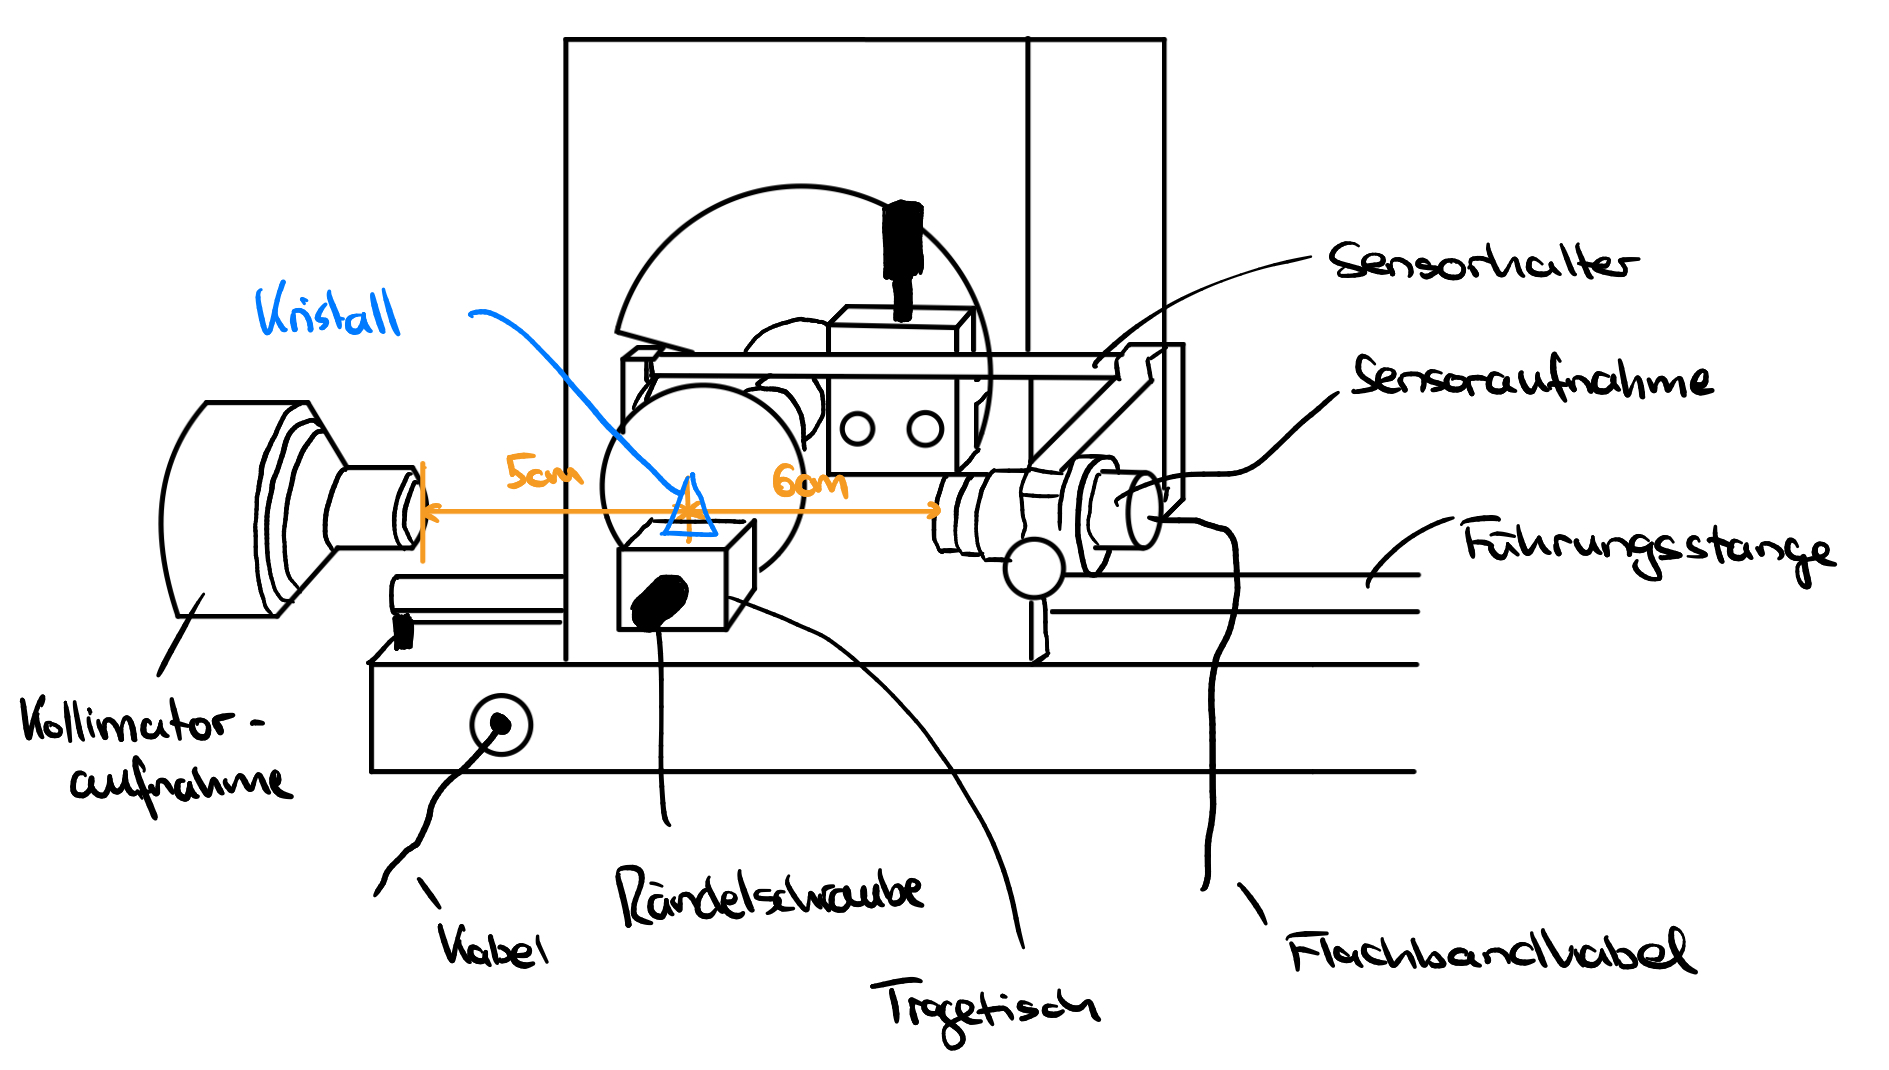
\includegraphics[width=0.7\linewidth]{Abbildungen/Aufbau Bragg Versuche.jpeg}
        \caption{Versuchsskizze Teilversuch 2}
        \end{figure}

    \item Planung der Durchführung
        \begin{itemize}
           \item Messreihe aus Teilversuch 1 löschen
           \item Folgende Einstellungen wählen: $I=1.00mA$, $\Delta t=10s$ und $\Delta\beta=0.1°$
           \item Targetwinkel einstellen auf: $\beta_{min}=2.5°$ und $\beta_{max}=12.5°$ $\to$ $2\vartheta$-Kopplung von Target und Sensor
           \item Röhrenhochspannung $U=20.0kV$ wählen und Messung und Datenübertragung an PC starten
           \item Zusätzliche Messreihe mit folgenden Werten durchführen: $U=25.0kV$, $\beta_{min}=2.5°$ und $\beta_{max}=18.0°$
           \item Laden der Messreohe mit $U=35.0kV$ mit Taste F3
           \item Dialogfenster (F5) öffnen und Gitterabstand des NaCl eintragen
           \item Alle Messreihen zusammen abspeichern
        \end{itemize}

    \item Vorüberlegungen zur Durchführung \& Auswertung
        \begin{itemize}
            \item Messreihen laden
            \item Peakschwerpunkte über gesamt Breite berechnen
            \item Vergleich mit Messwerten aus Teilversuch 1
            \item Interpretation der Messungen
        \end{itemize}
        
\end{enumerate}


\newpage


\subsection{Teilversuch 3: Duane-Huntsches Verschiebungsgesetz}
\begin{enumerate}[label = (\Roman*)]
    \item Ziel: Nachweis des Duane-Huntschen Verschiebungsgesetzes
    
    \item Versuchsmethode: Quantitative Untersuchung der Minimalwellenlänge in Abhängigkeit der Beschleunigungsspannung; Nachweis des Duane-Huntschen Verschiebungsgesetzes und Bestimmung des Planckschen Wirkungsquantums.
    
    \item Versuchsskizze:
    
        \begin{figure}[H]
        \centering
        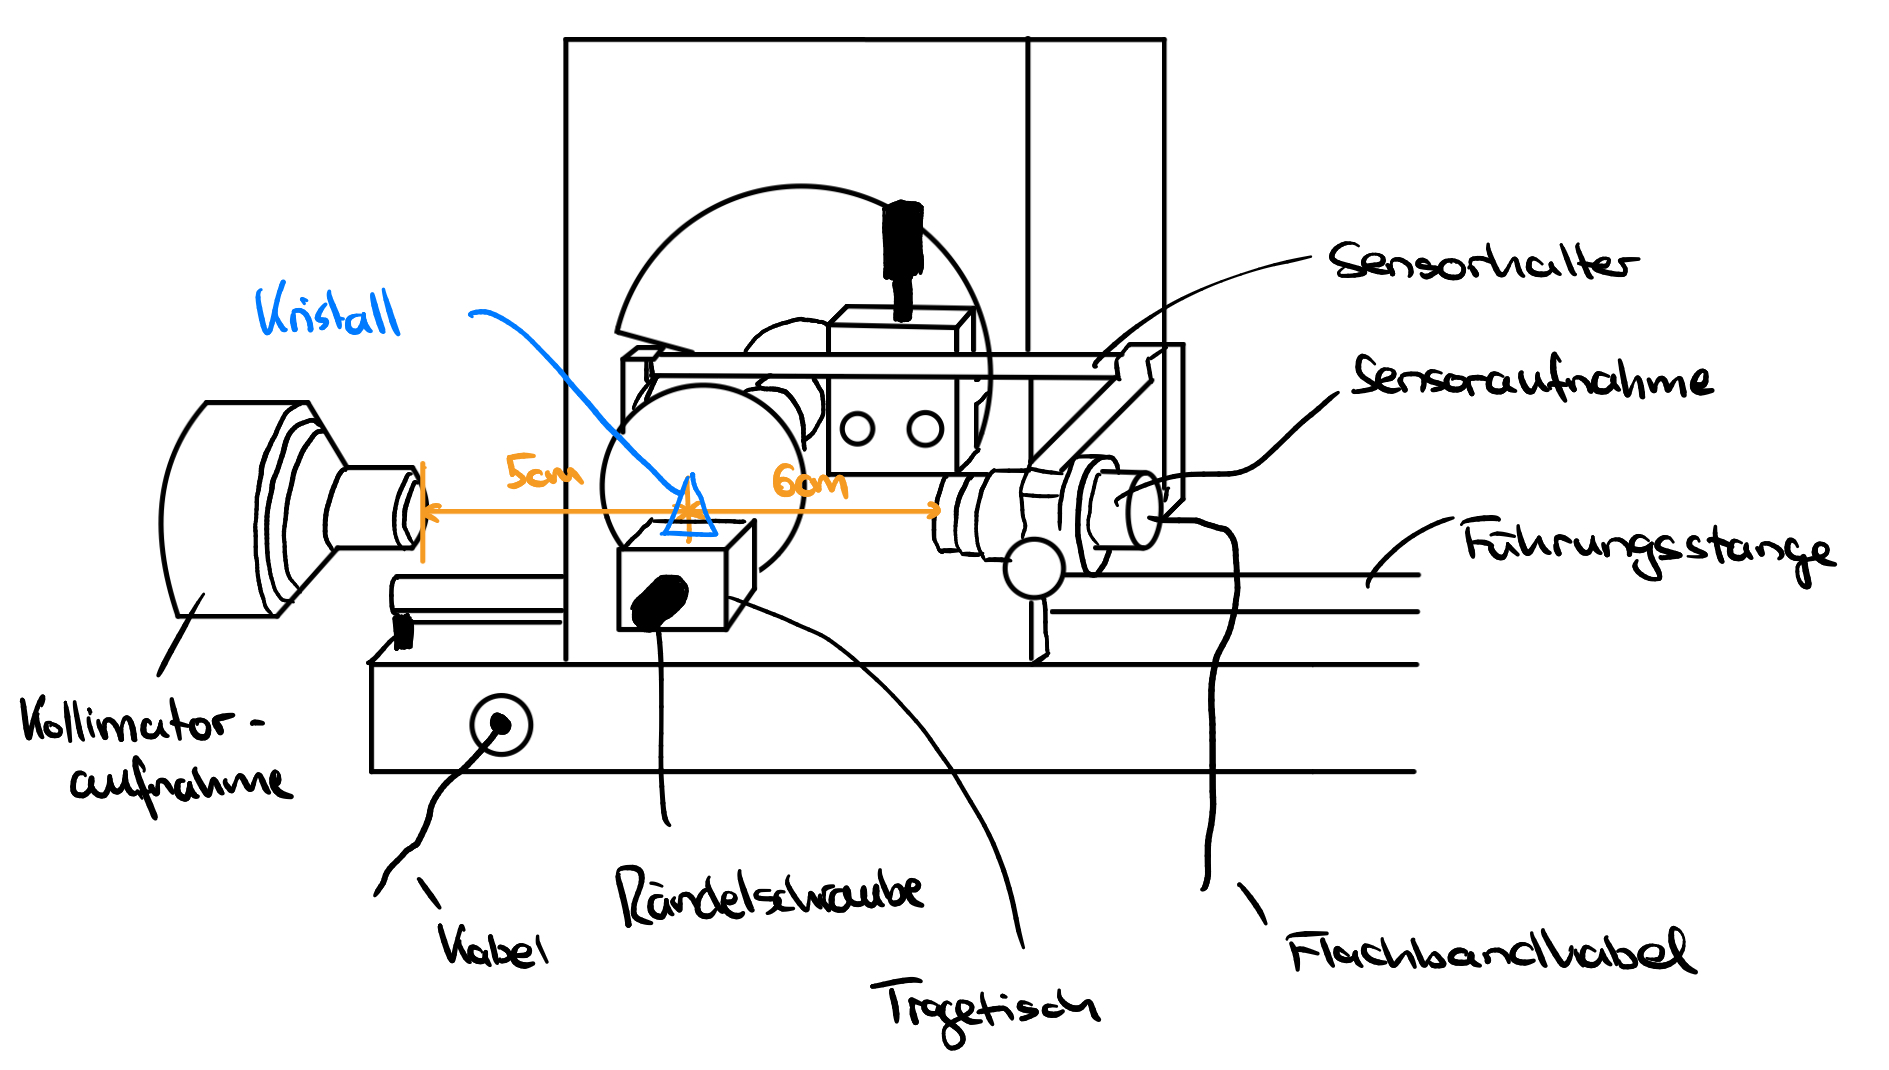
\includegraphics[width=0.7\linewidth]{Abbildungen/Aufbau Bragg Versuche.jpeg}
        \caption{Versuchsskizze Teilversuch 3}
        \end{figure}

    \item Planung der Durchführung
        \begin{itemize}
            \item Löschen der Messreihe aus Teilversuch 2
            \item Messreihe mit den Parametern aus folgender Tabelle aufnehmen:

            \begin{center}
                \begin{tabular}{ |c|c|c|c|c|c| } 
                 \hline
                 U [kV] & I [mA] & $\Delta t $ [s] & $\beta_{min}$ [grd] & $\beta_{max}$ [grd] & $\Delta\beta$ [grd] \\ 
                 \hline
                 22.0 & 1.00 & 30 & 5.2 & 6.2 & 0.1 \\ 
                 24.0 & 1.00 & 30 & 5.0 & 6.2 & 0.1 \\
                 26.0 & 1.00 & 20 & 4.5 & 6.2 & 0.1 \\
                 28.0 & 1.00 & 20 & 3.8 & 6.0 & 0.1 \\
                 30.0 & 1.00 & 10 & 3.2 & 6.0 & 0.1 \\
                 32.0 & 1.00 & 10 & 3.0 & 6.0 & 0.1 \\
                 34.0 & 1.00 & 10 & 3.0 & 6.0 & 0.1 \\
                 35.0 & 1.00 & 10 & 3.0 & 6.0 & 0.1 \\
                 \hline
                \end{tabular}
            \end{center}

            \item Dialogfenster öffnen und Gitterabstand des NaCl eintragen
            \item Messreihe anschließend speichern
        \end{itemize}

    \item Vorüberlegungen zur Durchführung \& Auswertung
        \begin{itemize}
            \item Überlegen, wie das Duane-Huntsche Verschiebungsgesetz mit simplen quantenmechanischen Überlegungen beschrieben werden kann
            \item Abhängigkeit zwischen Grenzwellenlänge und Röhren-Hochspannung beachten
            \item Unsicherheiten beachten!
            \item Bestimmen der Grenzwellenlänge $\lambda_{min}$ in Abhängigkeit von der Röhren-Hochspannung $U$ mit Computersoftware
            \item Bestätigung des Duane-Huntschen Verschiebungsgesetzes und Bestimmung des Planckschen Wirkungsquantums mit Computersoftware
        \end{itemize}
    
\end{enumerate}


\newpage


\subsection{Teilversuch 4: Röntgenfluoreszenzanalyse}
\begin{enumerate}[label = (\Roman*)]
    \item Ziel: Überprüfung des Moseleyschen Gesetzes und Bestimmung der Abschirmkonstanten
    
    \item Versuchsmethode: Aufnahme von Röntgenfluoreszenz-Spektren mehrerer Elemente; Energiekalibrierung und Überprüfung des Moseleyschen Gesetzes für die K-Linien des charakteristischen Spektrums; Bestimmung der Abschirmkonstanten für die Elektronen der K-Schalen, mittels Röntgen- fluoreszenz
    
    \item Versuchsskizze:
    
        \begin{figure}[H]
        \centering
        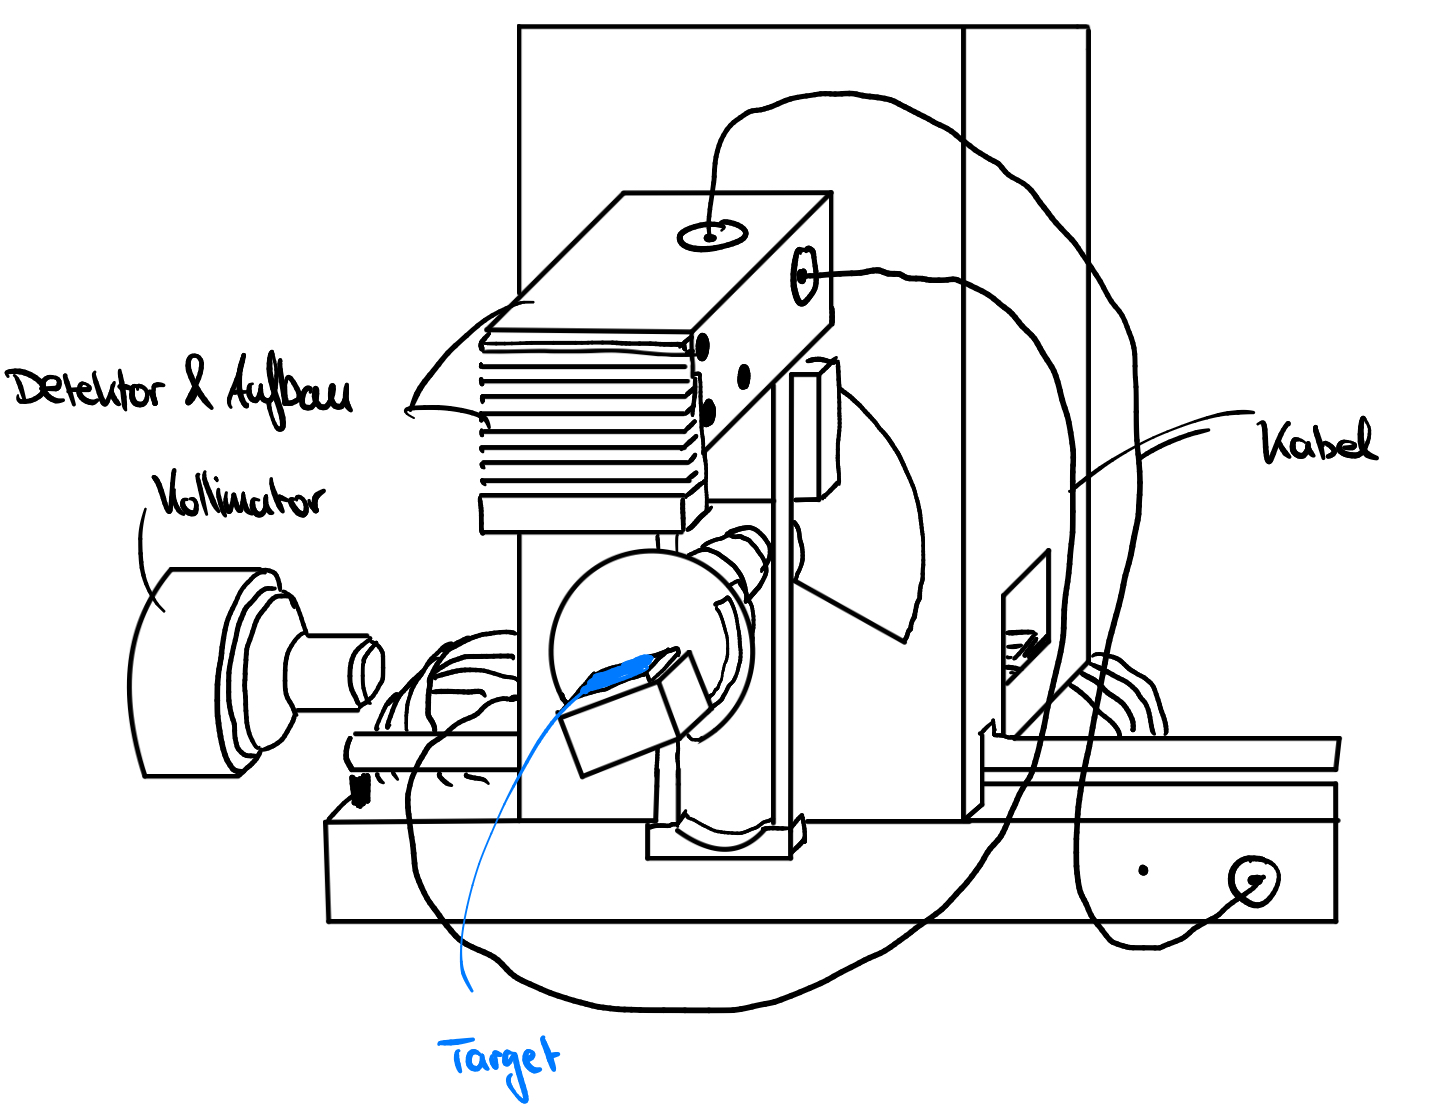
\includegraphics[width=0.7\linewidth]{Abbildungen/Aufbau Fluoreszenz.jpeg}
        \caption{Versuchsskizze Teilversuch 4}
        \end{figure}

    \item Planung der Durchführung
        \begin{itemize}
            \item Röntgengerät einschalten
            \item Durch Taste ZERO die automatische Einstellung auf 0 Grad vornehmen
            \item SENSOR drücken und Sensorwinkel mit ADJUST auf 90 Grad stellen
            \item TARGET drücken und Targetwinkel mit ADJUST auf 45 Grad stellen
            \item Tischnetzgerät an Netz anschließen (2 Minuten Wartezeit)
            \item Einstellen von CASSY-Lab. Folgende Punkte müssen beachtet werden: Vielkanalmessung, 512 Kanäle, negative Pulse, Verstärkung = -2.5, Messdauer = 180s
            \item Einstellungen am Röntgengerät: $U=35kV$, $I=1.00mA$
            \item K-Linien-Fluoreszenz auf den Tragetisch legen
            \item Hochspannung einschalten
            \item Spektrumaufnahme starten; Beobachten, wie sich das Spektrum aufbaut
            \item Anschließend Messung speichern und ausdrucken
            \item Nächstes Probeobjekt einlegen und Messung erneut durchführen
            \item Energiekalibrierung mit Eisen und Molybän durchführen!
        \end{itemize}

    \item Vorüberlegungen zur Durchführung \& Auswertung
        \begin{itemize}
            \item Schutzscheiben müssen geschlossen sein!
            \item Hochspannung immer ausschalten, wenn man das Probeobjekt ändert
            \item Bestimmen der Energien der einzelnen Linien
            \item Verhalten der Abschirmkonstanten analysieren
            \item War das zu erwarten und was sind Folgerungen?
        \end{itemize}
    
\end{enumerate}


\newpage


\subsection{Teilversuch 5: Identifiaktion einer unbekannten Probe mittels Röntgenfluoreszenz}
\begin{enumerate}[label = (\Roman*)]
    \item Ziel: Analyse des Stoffe des Probeobjekts
    
    \item Versuchsmethode: Mittels Röntgenfluoreszenz werden die Bestandteile einer unbekannten selbst mitge- brachten Probe bestimmt.
    
    \item Versuchsskizze:
    
        \begin{figure}[H]
        \centering
        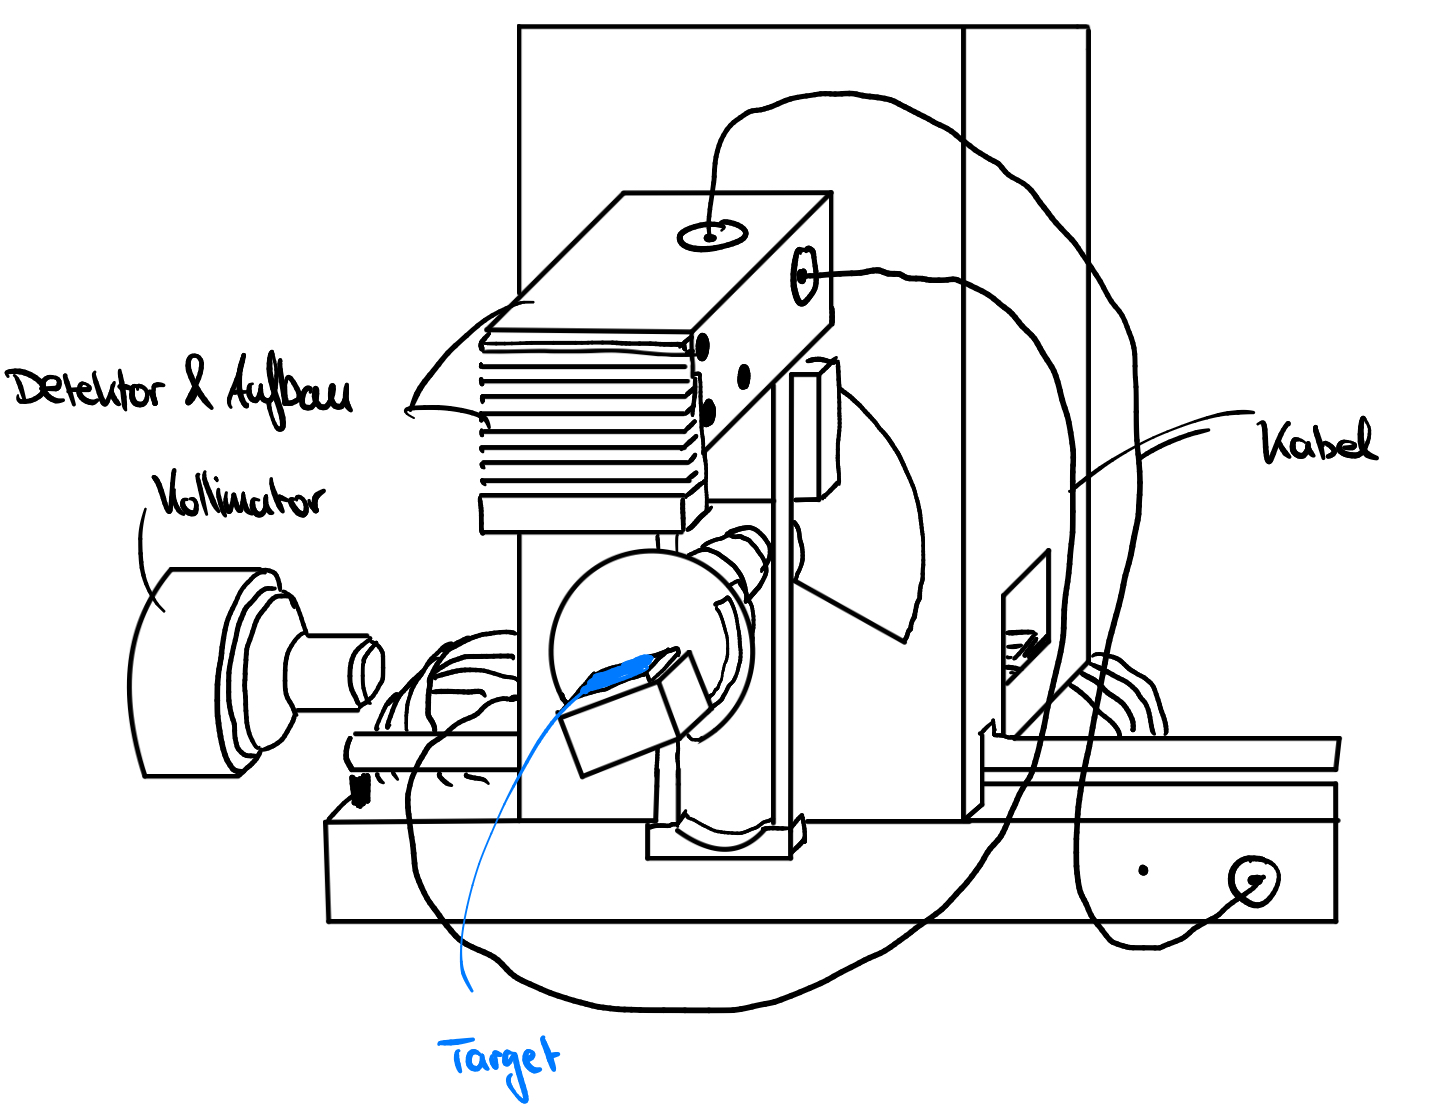
\includegraphics[width=0.7\linewidth]{Abbildungen/Aufbau Fluoreszenz.jpeg}
        \caption{Versuchsskizze Teilversuch 5}
        \end{figure}

    \item Planung der Durchführung
        \begin{itemize}
            \item Nach den Schritten aus Teilversuch 4 das Spektrum des Probekörpers aufnehmen
            \item Analyse des Objekts mit Hilfe des Periodensystems
            \item Zusammensetzung notieren
        \end{itemize}

    \item Vorüberlegungen zur Durchführung \& Auswertung
        \begin{itemize}
            \item Analyse, weshalb man genau auf diese Zusammensetzung gekommen ist
            \item Beleg mit Messdaten und Vergleichsdaten aus dem Periodensystem
        \end{itemize}
    
\end{enumerate}

\newpage

\iffalse

\section{Versuchsprotokoll}

Auf den folgenden Seiten befindet sich das eingescannte Versuchsprotokoll. Alle Daten wurden selbst gemessen. Sofern fremde Hilfe benutzt wurde, wurde sie klar gekennzeichnet.

Messunsicherheiten wurden angegeben und folgend in der Auswertung verwendet. Alle weiteren Rechnungen und Analysen finden in der Versuchsasuwertung statt.

\includepdf[pages={...}, pagecommand={\thispagestyle{scrheadings}}, frame=true]{[Name.pdf]]}

\newpage

\section{Auswertung}

    \subsection{Teilversuch 1: Bragg-Reflexion von Röntgenstrahlung des Molybdän an einem NaCl-Eiskristall}

    \newpage

    \subsection{Teilversuch 2: Energiespektrum einer Röntgenröhre in Abhängigkeit der Spannung}
    
    \newpage

    \subsection{Teilversuch 3: Duane-Huntsches Verschiebungsgesetz}

    \newpage

    \subsection{Teilversuch 4: Röntgenfluoreszenzanalyse}

    \newpage

    \subsection{Teilversuch 5: Identifiaktion einer unbekannten Probe}

    \newpage

\newpage

\section{Anmerkung: Graphische Auswertung und Fehlerfortpflanzung mit Python-Code}

Alle Berechnungen inkl. Fehlerbestimmung wurden mit einem selbstgeschriebenen
Python-Skript durchgeführt, um uns die Arbeit zu erleichtern und Fehler zu
vermeiden. Alle Ergebnisse, die auf diese Weise zustande gekommen sind,
sind entsprechend mit einem \colorbox{codebg}{blauen Hintergrund} gekennzeichnet;
s. folgendes Beispiel:
\[
    F \wideeq ma \wideeq \result{20}{kg} \cdot 9,81 \, \frac{\text m}{\text s^2}
    \wideeq \result{(19,62 \pm 0,5)}{N} \coderef{tv1}
\]
Dies soll bedeuten, dass die Berechnung des Wertes und der Unsicherheit von der
Python-Funktion namens \verb|tv1| durchgeführt wird.
Die Unsicherheit wird mithilfe der Gauß'schen Fehlerfortpflanzung berechnet.
Außerdem wird das Python-Package \texttt{matplotlib} zum Erstellen
von Graphen verwendet.

Der verwendete Code ist sowohl auf GitHub verfügbar (\githuburl) als auch auf den
folgenden Seiten zu finden und kann mit dem Befehl \texttt{python Main.py}
ausgeführt werden. Für eine genauere Beschreibung des Codes siehe die README-Datei
auf GitHub sowie die Kommentare im Code.
(Manche Sonderzeichen im Code (ä, ö, ü, $\Delta$, etc.) werden von \LaTeX nicht
richtig erkannt, deswegen kann der Code auf den nachfolgenden Seiten an einigen
Stellen unvollständig erscheinen. Auf GitHub wird aber alles richtig angezeigt.)

\newpage


\verb|Main.py|:
\lstinputlisting[language=Python]{Code/Main.py}
\newpage

\verb|Expressions.py|:
\lstinputlisting[language=Python]{Code/Expressions.py}
\newpage

Output:
\lstinputlisting{Code/Output.txt}

\fi

\end{document}